\documentclass{article}
\usepackage{nips12submit_e,times}
\usepackage{tikz}
\tikzstyle{vertex}=[auto=left,circle,fill=black!25,minimum size=20pt,inner sep=0pt]
\usepackage{verbatim}
\usepackage{url}
\usepackage{graphicx, color}
\usepackage{amsmath}
\usepackage{caption}
\usepackage{subcaption}
\usepackage{footnote}


\title{Stochastic Blockmodels for Relational Event Data} 

\author{
David S.~Hippocampus\thanks{ Use footnote for providing further information
about author (webpage, alternative address)---\emph{not} for acknowledging
funding agencies.} \\
Department of Computer Science\\
Cranberry-Lemon University\\
Pittsburgh, PA 15213 \\
\texttt{hippo@cs.cranberry-lemon.edu} \\
\And
Coauthor \\
Affiliation \\
Address \\
\texttt{email} \\
\AND
Coauthor \\
Affiliation \\
Address \\
}


\begin{document} 

\maketitle

\savenotes

\begin{abstract}
Observing network data as a stream of relational events provides an opportunity to understand differences in how nodes interact given the past.  For continuous-time network data, recent methods model the rate of dyadic events conditioned on the observed history of events and covariates about the nodes.  For static networks, methods such as stochastic blockmodels often account for node-level heterogeneity by assuming latent groups of individuals have similar tendencies in their group-wise interactions.  We propose to combine these two approaches by modeling the event dynamics within and between clusters of nodes.  The method is illustrated using dyadic interaction data such as email and Twitter direct messages.  Parameter estimates from the model clearly reveal heterogeneity in the dynamics among groups of individuals.  The fitted models have better predictive accuracy than baselines and relational event models without the latent structure.  Our approach illustrates the efficacy of combining a detailed model for local dependencies and a latent variable model for meso-scale dependencies.
\end{abstract}

\section{Introduction}

Statistical methods for analyzing network data have become increasingly useful for studying  phenomenon ranging from people communicating online to protein interactions \cite{Goldenberg2009}.  Stochastic blockmodels \cite{Nowicki2001, Kemp, Ishiguro2010} are a class of statistical models for static network data that employ latent variables to model unobserved heterogeneity by 1) assuming each node in the network belongs to some block (or cluster) and 2) parameterizing the probability of edges between nodes of each block.  % Such approaches are especially useful for large-scale network data where higher-order dependencies can cause models such as exponential random graph models to be too complex to fit.
% TODO: Cite Rodriguez: Modeling dynamics of social networks via h. blockmodels

Network data, however, is often collected as a sequence of events occurring over time.   Recent work leverages  continuous-time models from event history analysis  \cite{AalenOddO.2008} to model network-based event data \cite{Butts2008,Brandes2009,Perry2011,Stadtfeld2010,Stadtfeld2011,Opsahl2011,Vu2011,Vu2011a}.  These models allow one to specify how the process depends on the previous history of events.  In this way one may investigate theories about the underlying processes and make predictions about future data conditioned on the past.

The above continuous-time network models assume all nodes in the network behave according to identical dynamics.  In many cases this is unrealistic.  For example, in a small organization comprised of several teams, each team may uncover different patterns for collaborating via email --- individuals in one group may respond more quickly, while another group may preferentially send to highly active individuals.  

%, and in many cases emails between one pair of individuals will not affect emailing behavior between a separate pair of individuals.

Borrowing from the intuition of stochastic blockmodels, we propose a hierarchical model of continuous time network data that assumes latent clusters of nodes share similar patterns of interaction.  The behavior of the model is illustrated with simulated data.  We describe parameter estimation and the learning of the latent cluster assignments via MCMC.  Using data sets of dyadic communication among people, we compare the predictive performance of the fitted models to standard baselines.  Finally we show that the parameter estimates exhibit an interpretable structure to the event dynamics, sometimes identifying particular \emph{roles} of communication.
  
\section{Model}

%Each interaction then has a set of periods $d \in D_{ij}$ each with a start time $a_d$, an end time $b_d$, and a rate $\lambda_d$.
%Consider a nonhomogeneous Poisson process with  intensity $\lambda(t)$ that is piecewise constant with respect to a set of knots $\tau$.  We can then write the likelihood of $M$ events $\mathcal{A} = (t_1, \ldots, t_M)$ with $t_m > 0$ as
Consider a sequence of events $\mathcal{A} = (0,t_1, \ldots, t_M)$ arising from a nonhomogeneous Poisson process with  intensity $\lambda(t)$.  If the intensity is left continuous and piecewise constant with respect to a set of knots $\tau$ then the likelihood can be written
\begin{align}
\mathcal{L}(\mathcal{A}|\theta) &= \prod_{m=1}^M \lambda(t_m) \exp\left\{ - \int_{0}^{t_M} \lambda(s)ds \right\} \notag  \\
&= \prod_{m=1}^M \lambda(t_m) \prod_{k=1}^{|\tau|} \exp\left\{ - (\tau_{k} - \tau_{k-1}) \lambda(\tau_k) \right\}%  \exp\left\{ - (t - \tau_{M}) \lambda(t) \right\}
\end{align}
%\noindent where the $m$th event occurs at time $t_m$, the intensity function $\lambda(t)$ is left continuous, and each $\tau_k \in [0,t_M]$.

% \begin{align}
% \mathcal{L}(A|\theta) &= \prod_{m=1}^M \lambda_{i_m}(t_m|\cdot) \prod_{i \in \mathcal{R}}  \exp\left\{ - \int_{0}^{t_M} \lambda_{i}(\tau | \cdot)d\tau \right\} \\
% &= \prod_{m=1}^M \lambda_{i_m}(t_m|\cdot) \prod_{i \in \mathcal{R}} \prod_{v \in D_{i}} \exp\left\{ - (b_v - a_v) \lambda_{i}(b_v | \cdot ) \right\}
% \end{align}

One can extend the above to marked point processes where each event contains additional information.  In the context of relational events occurring among $N$ nodes, each event in the process contains both a sender $i$ and a recipient $j$ such that  $(i,j) \in \mathcal{R}$, where $\mathcal{R}$ is the \emph{risk set} comprised of all allowed dyads.  We assume each dyad $(i,j) \in \mathcal{R}$ occurs as a Poisson process with intensity $\lambda_{ij}(t|\cdot)$ that is piecewise constant and depends on the previous history of events  $\mathcal{A}_t = \{(t_m,i_m,j_m): t_m \in [0,t) \}$.  The likelihood of an observed event history $\mathcal{A}_{t_M}$ (also denoted $\mathcal{A}$ for convenience) is
\begin{align}
\mathcal{L}(\mathcal{A}|\theta) &= \prod_{m=1}^M \lambda_{i_m,j_m}(t_m|\cdot) \prod_{(i,j) \in \mathcal{R}}\exp\{ - (t_m - t_{m-1}) \lambda_{ij}(t_m | \cdot) \}
\label{eqn:llk}
\end{align}
%\prod_{(i,j) \in \mathcal{R}}\exp\{ - (t - t_{M}) \lambda_{ij}(t | \cdot) \}.

\begin{figure}
\centering 
\begin{minipage}[b]{0.45\linewidth}
  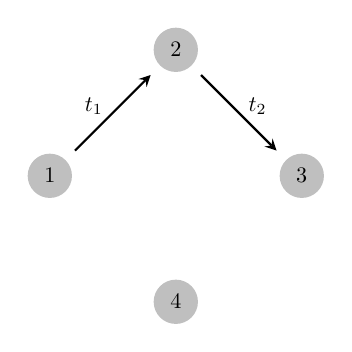
\begin{tikzpicture}[scale=.8,transform shape,thick]
    \node[vertex] (n1) at (0,0)  {1};
    \node[vertex] (n2) at (2,2)  {2};
    \node[vertex] (n3) at (4,0) {3};
    \node[vertex] (n4) at (2,-2) {4};
    \draw[-stealth] (.4,.4) -- (1.6,1.6);
    \draw[-stealth] (2.4,1.6) -- (3.6,.4);
    \node at (.7,1.1) {$t_1$};
    \node at (3.3,1.1) {$t_2$};
  \end{tikzpicture}
  \caption{Dynamic network data}
\end{minipage}
\begin{minipage}[b]{0.45\linewidth}
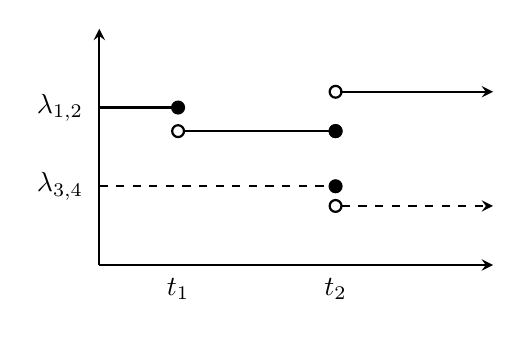
\begin{tikzpicture}[scale=1,transform shape,thick]
\draw[-stealth] (0,0) -- (0,3);
\draw[-stealth] (0,0) -- (5,0);

% First timeline
\draw (0,2) -- (1,2);
\draw[fill=black] (1,2) circle (0.75mm);
\draw (1,1.7) circle (0.75mm);
\draw (1.08,1.7) -- (3,1.7);
\draw[fill=black] (3,1.7) circle (0.75mm);
\draw (3,1.7) circle (0.75mm);
\draw (3,2.2) circle (0.75mm);
\draw[-stealth] (3.05,2.2) -- (5,2.2);

% second timeline
\draw[dashed] (0,1) -- (3,1);
\draw[fill=black] (3,1) circle (0.75mm);
\draw (3,.75) circle (0.75mm);
\draw[dashed, -stealth] (3.08,.75) -- (5,.75);

% labels
\node at (-.5,2) {$\lambda_{1,2}$};
\node at (-.5,1) {$\lambda_{3,4}$};
\node at (1,-.3) {$t_1$};
\node at (3,-.3) {$t_2$};
\end{tikzpicture}
\caption{Intensities for two dyads}
\end{minipage}
\caption[]{Illustration of event data and the assumptions of the model.  Left: An sequence of two events among four nodes: (1,2) occurs at time $t_1$ and (2,3) occurs at time $t_2$.  Right: The intensity functions $\lambda_{1,2}(t)$ (solid) and $\lambda_{34}(t)$ (dotted).  We assume $\lambda_{34}$ can only change after events sent or received by node 3.\footnotemark }
\label{fig:example}
\end{figure}

\footnotetext{TODO? Illustration of the block model, where events in cluster 1 (circles) are governed by the vector $\beta_{1,1}$, events in cluster 2 (squares) are governed by $\beta_{2,2}$, and an circle-to-square event governed by $\beta_{1,2}$.}


% \begin{figure}
%  \def\svgwidth{6in}
%   \input{example1.pdf_tex}
% \caption{Illustration of event data and the assumptions of the model.  Left: An sequence of two events among four nodes: (1,2) occurs at time $t_1$ and (2,3) occurs at time $t_2$.  Center: The intensity functions $\lambda_{1,2}(t)$ (solid) and $\lambda_{34}(t)$ (dotted).  Note $\lambda_{34}$ can only change when events occur involving either node 3 or node 4.  Right: Illustration of the block model, where events in cluster 1 (circles) are governed by the vector $\beta_{1,1}$, events in cluster 2 (squares) are governed by $\beta_{2,2}$, and an circle-to-square event governed by $\beta_{1,2}$.}
% \label{fig:example}
% %\includegraphics[width=6in]{example}
% \end{figure}

%This implies that  $\mathcal{R}_{i,j}$ is the set of dyads involving either $i$ or $j$ and that we will only use  statistics $\mathbf{s}(t,i,j)$ that do not change until an event involving either $i$ or $j$ occurs.  

We aim to learn about the dynamics between subsets of nodes.   To facilitate this, we assume each node $i$ is assigned a latent cluster $z_i$ and use a log linear model for the intensity functions
\begin{align*}
\log \lambda_{ij}(t | \mathcal{A}_t,\mathbf{\beta},\mathbf{z}) &= \boldsymbol{\beta}'_{z_i,z_j} \mathbf{s}(t,i,j,\mathcal{A}_t)
%z_i &\sim \mbox{CRP}(\alpha) &
%\boldsymbol{\beta}_{k,l} &\sim %\mbox{N}_p(\boldsymbol{\mu},\boldsymbol{\sigma}^2I)
\end{align*}
where for each pair of clusters $(k,l)$ we have a vector of parameters $\boldsymbol{\beta}_{k,l} \sim \mbox{N}_P(\boldsymbol{\mu},\boldsymbol{\sigma}^2I)$ that corresponds to the vector of $P$ statistics $\mathbf{s}(t,i,j,\mathcal{A}_t)$ computed from the previous history $\mathcal{A}_t$.  Thus, our model for the rate of $(i,j)$ events has the same parameters as for other dyads occurring between group $z_i$ and $z_j$.  

 In practice we may believe an interaction between one dyad should not affect the rate of an entirely separate dyad.  As shown in Figure \ref{fig:example}, we allow each intensity function $\lambda_{ij}(t)$ to only change following an event where $i$ was the sender or the recipient.  This is sensible in distributed settings where $i$ has limited knowledge about interactions among other actors.  In the Appendix we show how this assumption also reduces the computational complexity of computing the above likelihood.\footnote{This is analogous to a Markov condition for this class of models.}

We allow the blocks to share information by placing a hierarchical prior on the collection of $\boldsymbol{\beta}_{k.l}$ where $\mu_p \sim N(0,1)$ and $\sigma_p^2 \sim \mbox{Inv-Gamma}(3,1)$.  The cluster assignments are given a non-parameteric priors $z_i \sim \mbox{CRP}(\alpha)$.

\subsection{Model specification}
  
\begin{table}[t]
\footnotesize
\center
\begin{tabular}{|l|l|}
\hline
Statistic & Formula \\
\hline
\hline
Intercept& $s_{0}(t,i,j) = 1$\\
Reciprocity (AB-BA)& $s_{1}(t,i,j) = I(i_m=i,j_m=j,i_{v_{mij}}=j,j_{v_{mij}}=i)$\\
Turn-continuing (AB-AY)& $s_{2}(t,i,j) =  I(i_m=i,j_m=j,i_{v_{mij}}=i,j_{v_{mij}}\ne j)$\\
Turn-taking (AB-BY)&$s_{3}(t,i,j) = I(i_m=i,j_m=j,i_{v_{mij}}=j,j_{v_{mij}}\ne i)$\\
%Turn-usurping (AB-XA)& $s_{7}(t,i,j) = I(i_m=i,j_m=j,i_{v_{mij}} \ne j,j_{v_{mij}}=i)$\\
%Turn-usurping (AB-XB)&$s_{8}(t,i,j) = I(i_m=i,j_m=j,i_{v_{mij}} \ne i,j_{v_{mij}}=j)$\\
Sender out-degree& $s_{4}(t,i,j) = f(\sum_{m:t_m<t} I(i_m=i) )$\\
Sender in-degree& $s_{5}(t,i,j) = f(\sum_{m:t_m<t} I(j_m=i) )$\\
Dyad count& $s_{6}(t,i,j) = f(\sum_{m:t_m<t} I(i_m=i,j_m=j) )$\\
%Receiver out-degree& $s_{3}(t,i,j) = f(\sum_{m:t_m<t} I(i_m=j))$\\
%Receiver in-degree& $s_{4}(t,i,j) = f(\sum_{m:t_m<t} I(j_m=j))$\\
\hline
\end{tabular}
\label{tab:stats}
\caption{Statistics used to specify intensity functions using the previous history $\mathcal{A}_t$.}
\end{table}



In Table \ref{tab:stats} we list the statistics we use in our experiments for  $\mathbf{s}(t,i,j)$.  Several statistics use $v_{mij} \in [0,M]$, the index of the last event where $(i,j)$ occurred.  % (n.b. $t_{v_{mij}} = \tau_{mij}$). 
If $(i,j)$ has never occurred, we set $v_{mij}=0$.  We include degree effects to model possible rich-get-richer phenomenon.  For example, a particular node sending often may indicate they will continue to be a sender in the future.  We normalize these counts by the number of events up until a dyad's prior changepoint.\footnote{This seems to avoid ``explosion'' when simulating from the model.  TODO: Explore the theory about these sorts of statistics.  Aalen has a few suggestions.} Other statistics could be of interest for particular substantive questions \cite{Butts2008,Vu2011}.  \footnote{Describe the form of $f()$.  Right now it is $f(x) = \log \frac{x+1}{m + N(N-1)}$.}

The next set of statistics are \emph{participation shift} effects inspired by research in conversational norms \cite{Gibson2003}.  For example, an AB-BA effect indicates an increased propensity for reciprocity.  The final set of effects allow one to model phenomenon such as triadic closure.  Though we use only the above statistics in our experiments, one may use any quantity or set of covariates about a given dyad that is computed using the previous history of events.  The only restriction is that the statistic may not change in value between each observed event.\footnote{This prevents one from using the number of events occurring in some previous time window, as in \cite{Gunawardana2011}.}

\subsection{Relation to other models}

Our formulation is reminiscent of the stochastic blockmodel \cite{Nowicki2001,Kemp} which models the probability of a dyad as $p(y_{ij}) =\mbox{logit}^{-1}( \eta_{z_i,z_j})$ where $\eta_{z_i,z_j}$ is interpreted as a mixing rate between group $z_i$ and group $z_j$.  In the proposed method, however, the blockmodel structure facilitates the study of intra-group and inter-group dynamics via a continuous-time network model.

The above framework generalizes several important special cases. For example,  using only the intercept statistic $s_0(t,i,j) = 1$ is analogous to the stochastic block model for static networks.  Under this model each dyad is a homogeneous Poisson process and all dyad intensities $\lambda_{i,j}$ within block $(z_i,z_j)$ have the same intensity, $\exp\{\boldsymbol{\beta}_{z_i,z_j}\}$.  As these intensities do not change under this specification, the likelihood simplifies to 
$$\mathcal{L}(\mathcal{A}|\beta) = \prod_{m=1}^M \lambda_{i_m,j_m} \prod_{(i,j) \in \mathcal{R}} \exp\{-t_M \lambda_{i,j}\}$$

Alternatively, if one models only the order of the events (ignoring the times at which they occur), the likelihood can be written as
\begin{align}
\mathcal{L}_{\mbox{mult}}(\mathcal{A}|\beta) = \prod_{m=1}^M \frac{\lambda_{i_m,j_m}(t_m | \cdot)}{\sum_{(i,j) \in \mathcal{R}} \lambda_{i,j}(t_m | \cdot)}.
\label{eqn:multllk}
\end{align}
The functional form is similar to conditional logit models used for discrete choice data \cite{McFadden1984}, though here the possible choices are all the dyads in $\mathcal{R}$.


\section{Inference}

We use Markov chain Monte Carlo to sample from the posterior distribution of our parameters.\footnote{TODO: Describe why EM is hard.} % Note that approaches such as EM are difficult since the form of the likelihood does not admit an analytic expression for the expected complete data log likelihood.

\subsection{Sampling $\mathbf{z}$ given $\boldsymbol{\beta}$ and $\mathcal{A}$ }

We use Gibbs sampling to sample the latent class assignments $\mathbf{z}$ from the conditional distribution
\begin{align*}
p(z_r | \mathbf{z}_{-r},\mathcal{A},\alpha,\boldsymbol{\beta}) \propto&  p(\mathcal{A}|\mathbf{z},\boldsymbol{\beta}) p(z_r | \mathbf{z}_{-r},\alpha) \\
p(\mathcal{A}|\mathbf{z},\boldsymbol{\beta}) \propto &
\prod_{m=1}^M \lambda_{i_m,j_m}(t_m|\cdot)^{\mathbf{1}[r \in \{i_m,j_m\}]}  \prod_{(i,j) \in \mathcal{R}_r} \exp \{ -(t_m - t_{m-1}) \lambda_{ij}(t_m|\cdot)\} 
\end{align*} 
where $\mathcal{R}_r = \{(i,j) \in \mathcal{R}: r \in \{i,j\}\}$ is the set of dyads involving node $r$.  Under a CRP($\alpha$) prior, we have $p(z_i = k | z_{-i},\alpha) = n_k $ and $p(z_i = \mbox{new} |  z_{-i},\alpha) = \alpha$ where $n_k$ is the number of nodes assigned to cluster $k$.  In our experiments we use $\alpha=0.1$ and use Algorithm 8 from \cite{Neal2001} with 5 extra clusters drawn from the prior.\footnote{I also tried out a prior for cluster sizes such that $n_k \sim \mbox{NegBinom}(3,N/K)$, where $K$ is chosen a priori.  This aims for similarly sized groups.}

\subsection{Sampling $\boldsymbol{\beta}$ given $\mathbf{z}$ and $\mathcal{A}$ }

For each block $(k,l)$ we need to sample the vector of parameters $\boldsymbol{\beta}_{k,l}$ from its posterior
\begin{align*}
p(\boldsymbol{\beta}_{k,l} | \mathcal{A}, \textbf{z}, \boldsymbol{\mu}, \boldsymbol{\sigma}) &\propto p(\boldsymbol{\beta}_{k,l} | \boldsymbol{\mu}, \boldsymbol{\sigma}) p( \mathcal{A}| \textbf{z}, \boldsymbol{\beta}) \\ 
p(\boldsymbol{\beta}_{k,l} | \mu, \sigma) &= \prod_{p=1}^Pp(\beta_{k,l,p}|\mu_p,\sigma_p^2)\\
p(\mathcal{A}|\mathbf{z},\boldsymbol{\beta}) &\propto \prod_{m=1}^M \lambda_{i_m,j_m}(t_m|\cdot)^{\mathbf{1}[(i_m,j_m) \in \mathcal{V}_{k,l}]} 
\prod_{(i,j) \in \mathcal{V}_{k,l}} \exp \{ -(t_m - t_{m-1}) \lambda_{ij}(t_m|\cdot)\}
\end{align*}
where $\mathcal{V}_{k,l} = \{(i,j): z_{i} \in \{k,l\} \ \mbox{or} \ z_{j} \in \{k,l\} \}$ is the set of dyads with a sender in group $k$ and a recipient in $l$.  This distribution is sampled using slice sampling.

\subsection{Sampling $\mu$  and $\sigma$ given $\beta$ }

The inverse gamma distribution is a conjugate prior to a Gaussian distribution with known location parameter, thus $\sigma$ can be sampled from the conditional distribution
\begin{align}
\label{eqn:gibbs.sigma}
\sigma_p^2 &| \boldsymbol{\beta}, \mu_p,  \alpha_{\sigma}, \beta_{\sigma} \sim
 \mbox{Inv-Gamma}\left(\alpha_{\sigma} + \frac{K^2}{2}, \beta_{\sigma} + \frac{1}{2} \sum_{k=1}^K\sum_{l=1}^K (\beta_{p,k,l} - \mu_p)^2\right).
\end{align}
Each parameter $\mu_p$ can be sampled from its conditional distribution given $\sigma_p^2$ and the parameters $\boldsymbol{\beta}$, 
\begin{align}
\label{eqn:gibbs.mu}
\mu_p | \boldsymbol{\beta},\sigma_p^2 &\sim \mbox{Normal}\left(\frac{1}{K^2}\sum_{k=1}^K \sum_{l=1}^K \beta_{p,k,l},\frac{ \sigma_p^2}{\sqrt{K^2}}\right).
\end{align}

\begin{figure}
\center
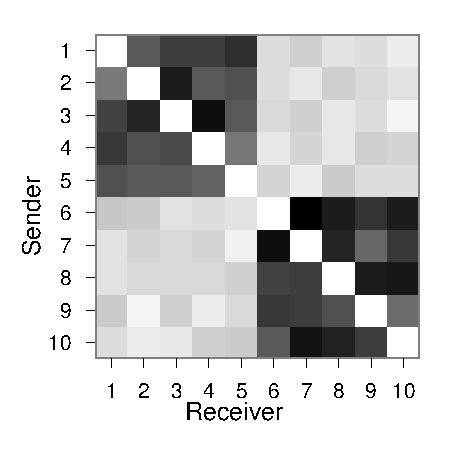
\includegraphics[width=1.6in]{../figs/synthetic/mat.pdf}
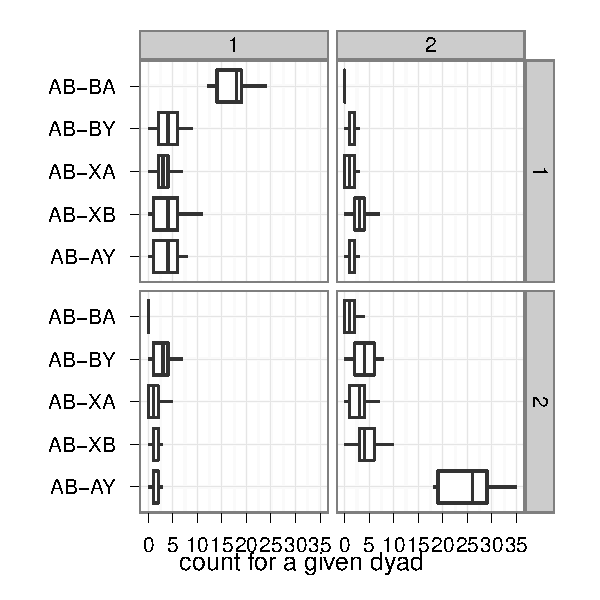
\includegraphics[width=2in]{../figs/synthetic/counts.pdf}
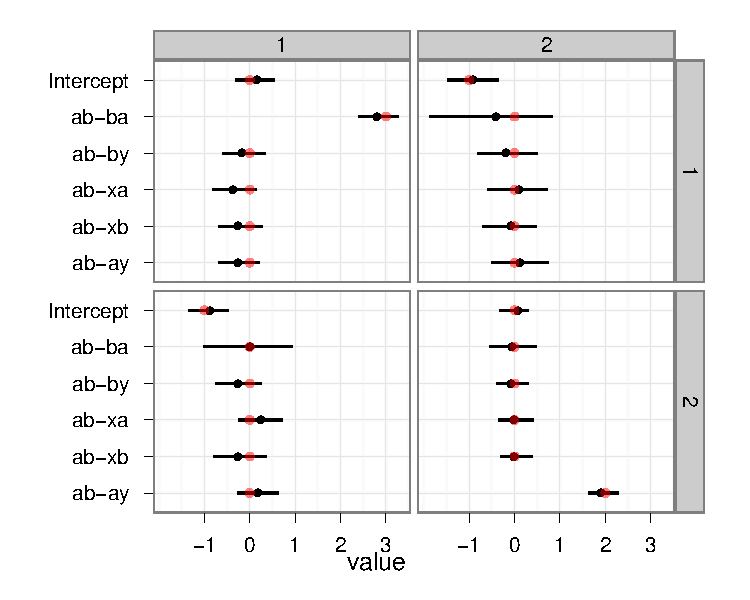
\includegraphics[width=1.8in]{../figs/synthetic/params-estimates.pdf}
\caption{Illustration of 2000 simulated events, as described in text. Left: Counts of each dyad. Center: Boxplot of distribution of participation counts across dyads.  The top left shows an increased propensity for reciprocity within cluster 1; bottom right shows more AB-AY events within cluster 2.  Right: Parameters (in red) and posterior credible intervals (in black).}
\label{fig:syncounts}
\end{figure}

\section{Simulation}

We check our model fitting procedure using a small synthetic data set involving 10 nodes from 2 clusters where 1) the first cluster has an increased tendency for reciprocity, 2) members of the second cluster have an increased tendency to subsequently talk to someone within their cluster.  The specification of $\textbf{s}$ is therefore $s(t,i,j) = [s_0, s_{1}(t,i,j), s_{2}(t,i,j)]$.  For the synthetic data set we use parameter vectors $\boldsymbol{\beta}_{1,1} = (0,3,0)$,  $\boldsymbol{\beta}_{1,2} = \boldsymbol{\beta}_{2,1} = (-1,0,0)$, and $\boldsymbol{\beta}_{2,2} = (0,2,0)$.  This is done by sequentially computing $\lambda_{ij}(t_m|\cdot)$ for all $(i,j) \in \mathcal{R}$, drawing $t_{m+1}-t_m \sim \mbox{Exp}(\sum_{ij} \lambda_{ij}(t_m|\cdot))$, and drawing the dyad $(i,j) \sim \mbox{Categorical}(\lambda_{ij}(t_m|\cdot) / \sum_{ij}\lambda_{ij}(t_m|\cdot))$.  

Though the dyad counts for the synthetic data set suggest a stochastic blockmodel (as seen in Figure  \ref{fig:syncounts}),  the center plot shows each block has empirical differences in their dynamics.  Intensities for reciprocal actions among nodes in block 1 are $e^3$ times greater, intensities for turn-taking actions among nodes in group 2 are $e^2$ times greater, and intensities for dyadic interactions between the two groups have a multiplicative effect of $e^{-1}$ and thus occur less often.  Fitting the model with $K=2$ has similar  predictive accuracy as the true model (see Table \ref{tab:results}), recovers the true latent classes, and the posterior credible intervals of the parameters cover the true parameter values (see Figure \ref{fig:syncounts}c).

\section{Model checking and experiments}

\subsection{Data}

Each of the following data sets are sequences of dyadic events, where each event has a time associated with it, a sender, and a recipient.

\begin{itemize}
%\item Kiel email: \cite{Ebel2002}
\item Classrooms: TODO describe datasets. Each have about 20 people and 400 events.  \cite{McFarland2003}
\item Eckmann email: dyadic emails.  2000 training events among 88 people and 1300 test events.  \cite{Eckmann}
\item Enron email: dyadic emails between months [TODO], 3000 training and 1000 test events among 141 actors \cite{Enron}
\item Irvine: dyadic interactions among 401 actors each having more than 30 events,  \cite{Opsahl}
\item Tweets from Twitter.com occurring between from May 11, 2009 to January 26, 2012 that contained the hashtag \texttt{\#rstats}.\footnote{Will be made publicly available.}  This hashtag is used to denote messages pertaining to the R statistical computing environment and sometimes statistical discussion more generally.  We collect dyadic events by selecting tweets beginning with the \texttt{@} symbol (called a \emph{mention}), and mark the first mentioned user as the recipient.  Of 28337 total tweets in this time period, 3926 were directed events among a total of 1079 users.  We use the subset of 487 users who participated in more than one event, using a training set of 2000 events and a test set of 1330 events.
\item MIT Reality Mining: phone calls among the 89 recipients between the dates , using of 2000 training events followed by 1000 test events. \cite{MITreality}
\end{itemize}

\subsection{Prediction experiments}

We evaluate the predictive ability of the fitted models by comparing models based on the loglikelihood of held-out data and recall on held out data.  Each data set is first split into a training set and a test set, and the loglikelihood of the test set is computed sequentially using Equation \ref{eqn:llk} where $\beta$ is set to be the mean from posterior samples given the training data.\footnote{This approach makes sense when the latent class assignments are not changing.  I will change this so that we averaging across predictions made from single draws from the posterior $\beta^{(i)}, z^{(i)}$.}   We compute both the relational event model likelihood  (\texttt{rem}) as given in Equation \ref{eqn:llk}  and the multinomial likelihood (\texttt{mult}) given in Equation \ref{eqn:multllk} .  The latter only measures a model's predictive performance for \emph{what} occurs next, while the former also measures the ability to predict \emph{when} it occurs.  

In addition, we compute recall to evaluate whether the next observed event is among the most likely according to the model.  At each event $m$ we sort the predicted intensities of all possible events in decreasing order, find the rank of the observed event in the list of predicted intensities, and compute the mean rank across the $M$ events.  

% latex table generated in R 2.15.0 by xtable 1.7-0 package
% Tue May 29 14:05:03 2012
\begin{table}[t]
\begin{center}
{\footnotesize
\begin{tabular}{llrrrrr}
  \hline
dataset & metric & uniform & marg & online & brem & truth \\ 
  \hline
synthetic-1 & rem & -0.741 & -0.741 & -0.400 & 0.192 & 0.196 \\ 
   & mult & -4.500 & -4.499 & -4.166 & -3.592 & -3.589 \\ 
  eckmann-small & rem & -8.764 & -7.729 & -6.661 & -6.652 &  \\ 
   & mult & -8.943 & -7.908 & -6.841 & -6.816 &  \\ 
  classroom-16 & rem & -4.863 & -2.876 & -2.482 & -2.040 &  \\ 
   & mult & -6.227 & -4.207 & -3.849 & -3.355 &  \\ 
  classroom-17 & rem & -5.134 & -4.388 & -3.557 & -3.558 &  \\ 
   & mult & -6.397 & -5.650 & -4.819 & -4.688 &  \\ 
  classroom-27 & rem & -5.379 & -3.837 & -3.320 & -3.290 &  \\ 
   & mult & -6.554 & -5.014 & -4.494 & -4.312 &  \\ 
  classroom-29 & rem & -5.310 & -3.139 & -3.104 & -4.304 &  \\ 
   & mult & -6.477 & -4.305 & -4.270 & -4.316 &  \\ 
  classroom-31 & rem & -5.563 & -3.942 & -3.766 & -3.895 &  \\ 
   & mult & -6.554 & -4.953 & -4.753 & -4.481 &  \\ 
   \hline
\end{tabular}
}
\caption{Comparing mean loglikelihood for each event across methods for each dataset.  Larger values are better.  See text for details.}
\label{tab:results}
\end{center}
\end{table}


\subsection{Baselines}

Several baselines are included for comparison: \texttt{uniform} places uniform probability on all possible dyads, \texttt{online} ranks events at time $t$ by the number of times the dyad has occurred previously $r_{online}(m,i,j) = \sum_{m:t_m < t} I(i_m=i,j_m=j)$, and \texttt{marginal} uses the product of the observed marginal frequencies $r_{marg}(m,i,j) = \sum_{m:t_m < t} I(i_m=i) \sum_{m:t_m < t} I(j_m=j)$.  Note for processes that are homogeneous over time, \texttt{online} should do well with large amounts of data while \texttt{marginal} should roughly model heterogeneity in activity among individuals.  

Our method jointly models \emph{which} dyads occur and \emph{when} they occur.  To compare the above baselines to our model using the likelihood of observed data, we assume each dyad is a Poisson process with estimated  rate $\hat{\lambda}_{i,j}(t_m) = \frac{M}{t_M} \frac{r_{b}(i,j) + \xi}{\sum_{ij} r_{b}(i,j) + \xi}$, where $r_b(i,j)$ is the statistic a baseline (described above) and $\xi=1$ is a smoothing parameter.


% latex table generated in R 2.15.0 by xtable 1.7-0 package
% Tue May 29 14:06:16 2012
\begin{table}[t]
\begin{center}
{\footnotesize
\begin{tabular}{llrrrrr}
  \hline
dataset & metric & uniform & marg & online & brem & truth \\ 
  \hline
synthetic-1 & @  5 & 0.060 & 0.077 & 0.113 & 0.443 & 0.438 \\ 
   & @ 20 & 0.226 & 0.304 & 0.447 & 0.684 & 0.674 \\ 
  eckmann-small & @  5 & 0.002 & 0.058 & 0.101 & 0.124 &  \\ 
   & @ 20 & 0.004 & 0.096 & 0.262 & 0.282 &  \\ 
  classroom-16 & @  5 & 0.000 & 0.356 & 0.582 & 0.671 &  \\ 
   & @ 20 & 0.014 & 0.610 & 0.808 & 0.822 &  \\ 
  classroom-17 & @  5 & 0.005 & 0.254 & 0.325 & 0.411 &  \\ 
   & @ 20 & 0.061 & 0.416 & 0.538 & 0.619 &  \\ 
  classroom-27 & @  5 & 0.000 & 0.331 & 0.428 & 0.490 &  \\ 
   & @ 20 & 0.014 & 0.517 & 0.724 & 0.669 &  \\ 
  classroom-29 & @  5 & 0.016 & 0.398 & 0.553 & 0.528 &  \\ 
   & @ 20 & 0.041 & 0.642 & 0.683 & 0.805 &  \\ 
  classroom-31 & @  5 & 0.008 & 0.322 & 0.322 & 0.483 &  \\ 
   & @ 20 & 0.017 & 0.407 & 0.525 & 0.669 &  \\ 
   \hline
\end{tabular}
}
\caption{Predictive accuracy on a recall task.  Larger values are better.  See text for details.}
\label{tab:results}
\end{center}
\end{table}


% \begin{figure}[t]
% \center
% \fbox{\rule[-.5cm]{0cm}{4cm} \rule[-.5cm]{4cm}{0cm}}
% \fbox{\rule[-.5cm]{0cm}{4cm} \rule[-.5cm]{4cm}{0cm}}
% \fbox{\rule[-.5cm]{0cm}{4cm} \rule[-.5cm]{4cm}{0cm}}
% \caption{Recall plots showing predictive performance on a ranking task.  Left: Eckmann.  Right: Another dataset.  (TODO)}
% \label{fig:recall}
% \end{figure}

\subsection{Results}

 Table \ref{tab:results} compares the train and test likelihood for each method and data set combination.  For the synthetic data generated with $K=2$ clusters, the model with $K=2$ is best as expected.  Fitting the model with a single cluster also outperforms the simple baselines with respect to both likelihoods.  

For the Eckmann subset the fitted model with $K=2$ performs best except for the test data using the conditional logit likelihood.  This may be because the model has overfit the training set, or the sampler has not properly converged (as is the case with $K=3$).  \footnote{Will need to discuss results for other datasets once they are complete.}

Figure \ref{fig:recall} will provide recall curves for several of the datasets.

\section{Discussion}

%% TODO: Discuss scalability.
%% TODO: Describe and include posterior predictive checks.

\begin{figure}[t]
\centering
\begin{subfigure}[b]{0.35\textwidth}
\centering
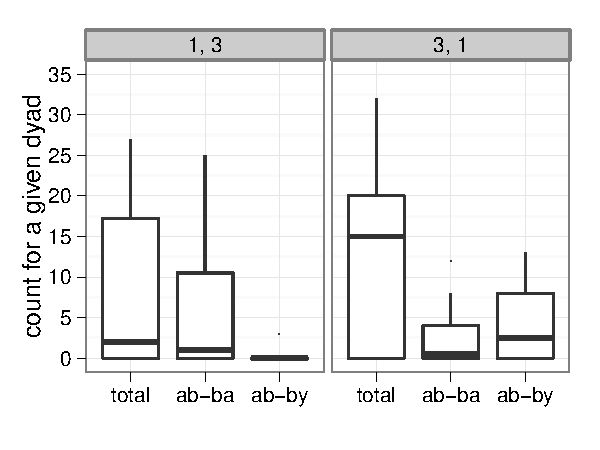
\includegraphics[scale=.5]{../figs/eckmann-small/example-obs-stats}
%\caption{Observed counts}
\end{subfigure}
\qquad
\begin{subfigure}[b]{0.35\textwidth}
\centering
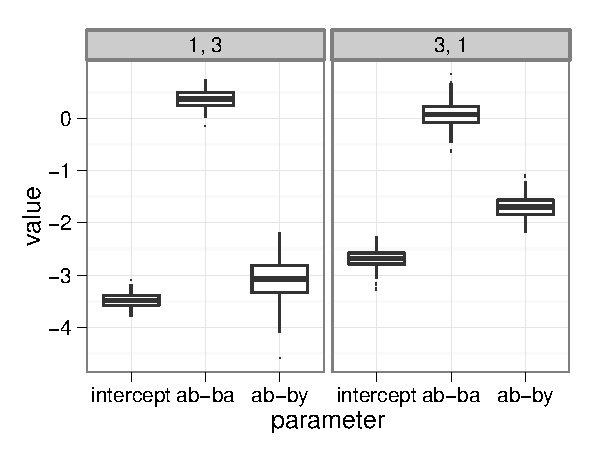
\includegraphics[scale=.5]{../figs/eckmann-small/example-estimates}
%\caption{Samples of $\beta_{p,k,l}$}
\end{subfigure}

\caption{%Observed counts versus model estimates from Eckmann email data.
 Left: Observed statistics across all dyadic email interactions from members of group 1 to group 3 (178 total events in total) and from members of group 3 to group 1 (179 events in total).  Right: Posterior samples of the corresponding $\beta_{p,1,3}$ and $\beta_{p,3,1}$.  In addition to finding differences in mean activity for these dyads, the model learns that events from 3 to 1 have a higher propensity for \texttt{ab-by} transitions.}
\label{fig:posteriorparams}
\end{figure}

\begin{figure}[t]
\centering
\begin{subfigure}[b]{0.22\textwidth}
\centering
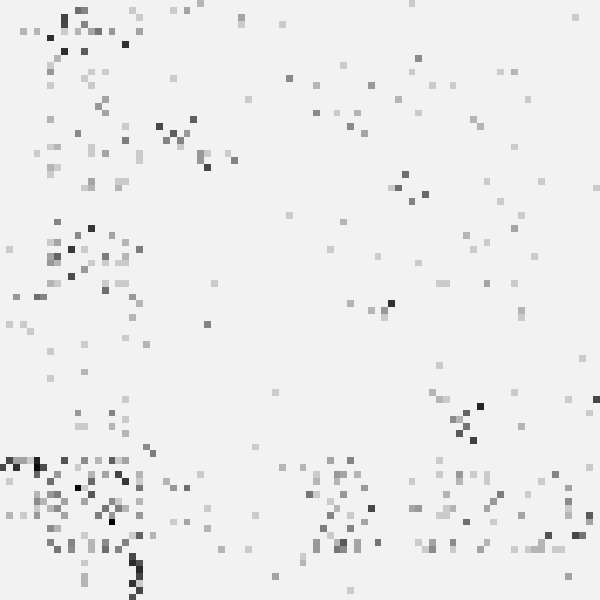
\includegraphics[scale=.25]{../figs/eckmann-small/parmat/observed}
\caption{Observed counts}
\end{subfigure}
~
\begin{subfigure}[b]{0.22\textwidth}
\centering
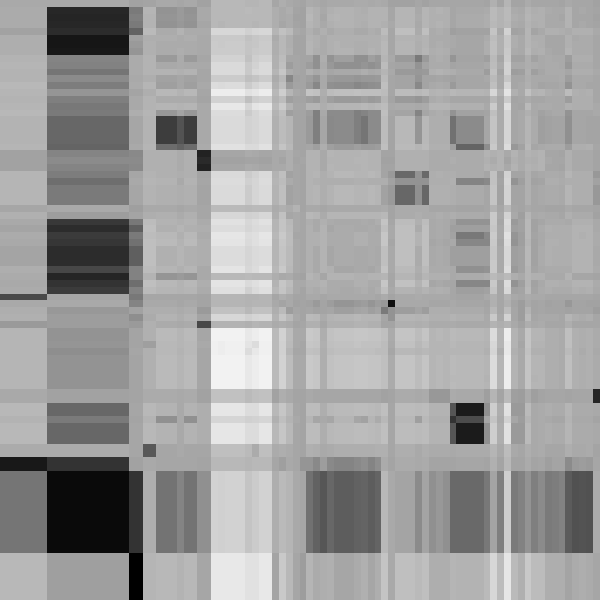
\includegraphics[scale=.25]{../figs/eckmann-small/parmat/1}
\caption{Intercept estimates}
\end{subfigure}
~
\begin{subfigure}[b]{0.22\textwidth}
\centering
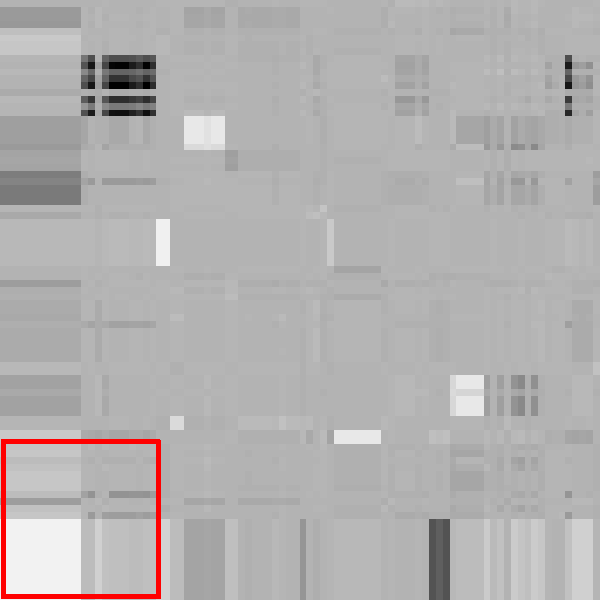
\includegraphics[scale=.25]{../figs/eckmann-small/parmat/2}
\caption{\texttt{ab-ba} estimates}
\end{subfigure}
~
\begin{subfigure}[b]{0.22\textwidth}
\centering
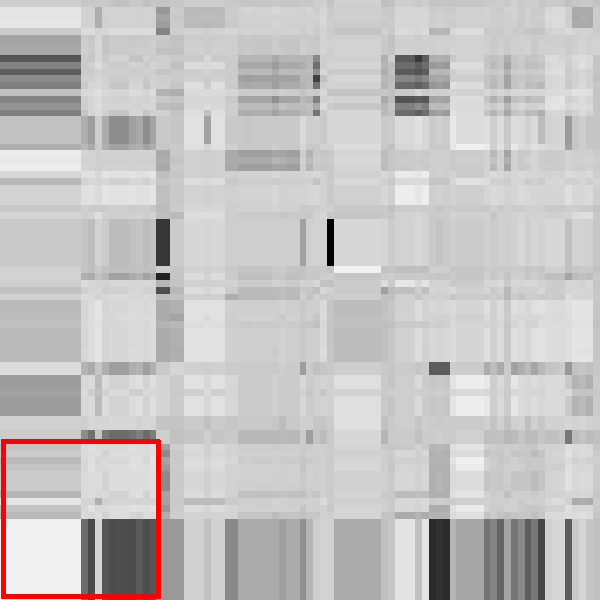
\includegraphics[scale=.25]{../figs/eckmann-small/parmat/3}
\caption{\texttt{ab-by} estimates}
\end{subfigure}
\caption{Comparing observed counts and parameter estimates.  Darker values are larger.  Estimates are rescaled posterior means $(\hat{\beta}_{p,z_i,z_j} - \hat{\mu}_p)/\hat{\sigma}_p$ for each dyad $(i,j)$.  Learned parameters suggest heterogeneity exists in both total activity (b) as well as dynamics, as seen in (c) and (d).}
\label{fig:parmats}
\end{figure}

 We propose a hierarchical approach for modeling event-based network data that is analogous to recent hierarchical extensions for latent position models \cite{Handcock2007} and exponential random graph models \cite{Schweinberger2011}.  The method combines a latent variable framework (stochastic blockmodels) with a local dependence model for event sequences (relational event models) to provide detailed models of event dynamics among subsets of nodes while allowing for heterogeneity in dynamics of the network as a whole.

Figure \ref{fig:posteriorparams} shows examples of model estimates from data sets of dyadic interactions for the Eckmann data. Panels contain posterior credible intervals for parameters pertaining to dyads belonging to a particular block.  

%For example, events among nodes in cluster 1 have an increased propensity for reciprocal events -- after node A sends to node B, an event from B to A has an intensity that is $e^4$ larger, all else held constant.  Interestingly, degree effects seem to vary by block: in block (2,2) active senders are more likely to be a sender whereas in block (1,1) the number of previous occurrences for a given dyad has a larger multiplicative effect.  

This analysis suggests key differences exist in typical behaviors or roles that subsets of nodes share.  Other theories could be explored by including relevant statistics in the specification of $\mathbf{s}(t,i,j,\mathcal{A}_t)$, and similarly one can use our method to study how the roles of these statistics vary across nodes.

In Section \ref{sec:experiments} we show the model has improved predictive accuracy over baseline methods on real data with respect to ranking tasks and the likelihood of unobserved data.  We also note that we improve over the situation where we constrain $K=1$.

Relational event models \cite{Butts2008} require a knot at each observed event, while other approaches such as \cite{Gunawardana2011} learn the regions where an intensity is constant.  By using decision trees,  \cite{Gunawardana2011} also allow for a nonlinear relationship between statistics and intensity functions, while here we use latent variables to allow for heterogeneity in intensities across possible events.

Trivially extended to co-clustering applications and for directed data.  Also useful for our model when nodes belong to one latent class as a sender but another latent class as a recipient.

Our method learns about event dynamics within latent groups of individuals, but other types of heterogeneity likely exist in some data sets.  For example, dynamics might change over time \cite{Vu2011}.  Alternatively, if nodes change groups.  One approach, analogous to \cite{Airoldi2008}, would allow the latent class $z_i$ to be drawn from node-specific membership vectors $\pi_i$  after each change point.  In some contexts such extensions might be substantively important and warrant future work.

\subsubsection*{Acknowledgements}

\bibliographystyle{unsrt}
\bibliography{refs}

\appendix{\textbf{Complexity}}

We take advantage of our restriction on the types of statistics $s$ to reduce the computational complexity of computing our likelihood
 Equation \ref{eqn:likelihood} as 
\begin{align*}
\mathcal{L}(\mathcal{A}_{t_M}|\theta) &= \prod_{m=1}^M \lambda_{i_m,j_m}(t_m|\cdot) \prod_{(i,j) \in \mathcal{R}_{i_m,j_m}}\exp\{ - (t_m - \tau_{mij}) \lambda_{ij}(t_m | \cdot) \}
\end{align*}
\noindent where event $m$ is the dyad $(i_m,j_m)$, $\tau_{mij}$ is the time  of the changepoint for $\lambda_{i,j}$ prior to the $m$th event, and $\mathcal{R}_{i,j}$ is the set of dyads whose intensity changes if $(i,j)$ occurs  \cite{Butts2008}. \footnote{We further assume 1) all intensity functions change at times $t=0$ and $t=t_M$, and 2) the first event is drawn uniformly from the risk set.}

 By limiting the changepoints to times when either node is involved, computing the likelihood $p(A|z,\beta,\mbox{node} \ r \ \mbox{involved})$ is $O(|\mathcal{U}_r| \cdot P \cdot N)$.  We precompute $\tau_{m,i,j}$ and $\mathbf{s}(t_m,i,j)$ for all $m$, $i$, and $j$. 

\appendix{\textbf{Split-merge Metropolis-Hastings move for non-conjugate stochastic blockmodels}}

%Motivation: simply Gibbs sampling does not seem to mix well.  \footnote{This section is planned future work. In the experiments we evaluate the performance of the model when restricting the number of clusters $K$.  For these chains we do not propose split moves when the number of non-empty clusters is already $K$.}

Here we describe a novel split-merge move for non-conjugate blockmodels.\footnote{IRM (modeling Bernoulli data with a conjugate Beta prior) used a split-merge algorithm \cite{Kempe2006}.}  For illustration, we consider the model
\begin{align*}
  y_{ij} & \sim \mbox{Poisson}(\Lambda_{z_i,z_j}) & \Lambda_{ij} &\sim \mbox{Gamma}(\alpha_{\Lambda},\beta_{\Lambda})  & z_i &\sim \mbox{CRP}(\gamma)
\end{align*}

IDEA: References are Dahl 2003, Wang, Blei 2012, Neal 2000 (alg 8).  A proposed split has REM parameters that are only slightly different than those for the original block.  Merges of two sets of REM parameters are performed by using the parameter for one blocks, and doing so for each dimension independently.  By keeping track of the probability of each of these transitions we can correctly compute the Metropolis-Hastings acceptance probability needed to guarantee we have an MCMC transition that leaves the posterior distribution invariant.


This is a two-stage MH procedure.  First, pick two nodes $i,j$ uniformly.  If they belong to the same block $k$ (i.e. $z_i=z_j=k$), then let the ``merge'' state $(\boldsymbol{\phi}^{m},\mathbf{z}^{m}) = (\boldsymbol{\phi},\mathbf{z})$ and propose a ``split'' state $(\boldsymbol{\phi}^{s},\mathbf{z}^{s})$ with new cluster $l$:
\begin{itemize}
\item Sample $\phi_{kk}^{s} \sim N(\phi_{kk}^{m},\sigma^2)$ and $\phi_{ll}^{s} \sim N(\phi_{kk}^{m},\sigma^2)$ and for blocks $r \ne l$, sample $\phi_{lr}^{s} \sim N(\phi_{kr}^{m},\sigma^2)$ and $\phi_{rl}^{s} \sim N(\phi_{rk}^{m},\sigma^2)$ 
\item For all $a$ such that $z_a^{m} = k$, randomly initialize $z_a^{s}$ to either $k$ or $l$, then perform a restricted Gibbs scan by sampling $p(z_{a}^{s}=k|\cdot)  \propto n_k p(A|\mathbf{z}^{s}_{-a},\boldsymbol{\phi}^{s})$
where $n_k=\sum_{i}I(z_i^{s}=k)$.% and compute $q( \mathbf{z}^{m} \rightarrow \mathbf{z}^{s})$ to be the product of the probabilities for the sampled assignments.
\item Accept  $(\boldsymbol{\phi}^{s},\mathbf{z}^{s})$ as the new state with probability $\alpha^*$, defined below.
\end{itemize}

 If $i$ and $j$ belong to different blocks $k$ and $l$ (i.e. $z_i = k \ne z_j=l$), we set the ``split'' state  $(\boldsymbol{\phi}^{s},\mathbf{z}^{s}) = (\boldsymbol{\phi},\mathbf{z})$ and propose a ``merge'' state $(\boldsymbol{\phi}^{m},\mathbf{z}^{m})$ as follows:
\begin{itemize}
\item Sample $\phi_{kk}^m \sim N((\phi_{kk}^s + \phi_{ll}^s)/2,
  \sigma^2)$.  Sample $\phi_{ll}^m \sim N(0,\tau^2)$ and for all blocks $r \ne k,l$ sample $\phi_{kr}^{m} \sim N(0,\tau^2)$ (the prior)
\item For all $a$ such that $z_a \in \{k,l\}$ set $z_a^m = k$.
\item Accept $(\boldsymbol{\phi}^{m},\mathbf{z}^{m})$ as the new state with probability $1/\alpha^*$, defined below.
\end{itemize}

 The Metropolis-Hastings acceptance probabilities require the quantity
$$\alpha^* =\frac{p(Y|\boldsymbol{\phi}^{s},\mathbf{z}^{s})}{p(Y|\boldsymbol{\phi}^{m},\mathbf{z}^{m})}  \frac{p(\boldsymbol{\phi}^{s})}{p(\boldsymbol{\phi}^{m})} \frac{p(\mathbf{z}^{s})}{p(\mathbf{z}^{m})} \frac{q(\mathbf{z}^{s} \rightarrow \mathbf{z}^{m})}{q( \mathbf{z}^{m} \rightarrow \mathbf{z}^{s})} \frac{q(\boldsymbol{\phi}^{s} \rightarrow \boldsymbol{\phi}^{m})}{q(\boldsymbol{\phi}^{m} \rightarrow \boldsymbol{\phi}^{s})}$$

The first term is the likelihood ratio of the two states.  Letting $S$ be the set of nodes assigned to $k$ or $l$ in $\mathbf{z}^{s}$, the probability of sampling $\mathbf{z}^{s}$ during a restricted Gibbs scan from  $\mathbf{z}^{m}$ is computed as $q( \mathbf{z}^{m} \rightarrow \mathbf{z}^{s}) = \prod_{s \in S} p(z_{s}=z_s^{s} |\{ z_a^{s},z_{b}^{m}: a  < s \ \mbox{and} \ s < b\}, \boldsymbol{\phi}^{s})$.  Since there is only one way of combining two clusters, we know $q(\mathbf{z}^{s} \rightarrow \mathbf{z}^{m})=1$.   The transition $q(\boldsymbol{\phi}^{m} \rightarrow \boldsymbol{\phi}^{s})$ and 
$q(\boldsymbol{\phi}^{s} \rightarrow
\boldsymbol{\phi}^{m})$ are products of Normal densities. \footnote{To ensure both states have the same dimensionality, one can optionally sample the parameters empty cluster $l$, though the extra term  in $q(\boldsymbol{\phi}^{s} \rightarrow \boldsymbol{\phi}^{m})$ would cancel with a corresponding term in $p(\boldsymbol{\phi}^{m})$}  Finally, under this prior $ \frac{p(\mathbf{z}^{s})}{p(\mathbf{z}^{m})} = \frac{(n_{z_i}^{s} - 1)!(n_{z_j}^{s} - 1)!}{(n_{z_i}^{m}-1)!}$.  

Since the proposed split vectors $\phi^s$ are close the $\phi^m$, this has a higher probability than the split states having arisen from the proposed merge state, which is closer to the midpoint between the two $\phi^s$ vectors.  This increases the acceptance probability for splits (and decreases the probability of merges).  However, the probability of getting assigned to each cluster (through the restricted Gibbs scan) might balance things out.

\spewnotes

\end{document}
